\documentclass{beamer}
\geometry{paperwidth=140mm,paperheight=105mm}
\usetheme{metropolis}           % Use metropolis theme
%\usetheme{CambridgeUS}
\title{Kolloquium zur Bachelorarbeit}
\subtitle{Untersuchung von Knotenreduktionsregeln beom Knoten{\"u}berdeckungsproblem}
\date{07. M{\"a}rz 2018}

\institute{Universit{\"a}t Trier}

%Pseudocode
\usepackage{listings}
\usepackage{lstlinebgrd}
\lstset{
  numbers=left,
  stepnumber=1,    
  firstnumber=0,
  numberfirstline=true,
extendedchars=true, literate=%
    {Ä}{{\"A}}1%
    {Ö}{{\"O}}1%
    {Ü}{{\"U}}1%
    {ä}{{\"a}}1%
    {ö}{{\"o}}1%
    {ü}{{\"u}}1%
    {ß}{{\ss}}1%
}
\usepackage[skip=1pt]{caption}
\usepackage{graphicx}
%Footer
\setbeamertemplate{footline}
{
  \leavevmode%
  \hbox{%
  \begin{beamercolorbox}[wd=.4\paperwidth,ht=2.25ex,dp=1ex,center]{author in head/foot}%
    \usebeamerfont{author in head/foot}Benedikt L{\"u}ken-Winkels
  \end{beamercolorbox}%
  \begin{beamercolorbox}[wd=.6\paperwidth,ht=2.25ex,dp=1ex,center]{title in head/foot}%
    \usebeamerfont{title in head/foot}\insertshorttitle\hspace*{3em}
    \insertframenumber{} / \inserttotalframenumber\hspace*{1ex}
  \end{beamercolorbox}}%
  \vskip0pt%
}

%Mathematikumgebungen
\usepackage{amsmath,amsthm,amssymb}
\usepackage{ngerman}
\usepackage[utf8]{inputenc}
\graphicspath{{img/}}

%Farbe für Block
\definecolor{amber}{rgb}{1.0, 0.75, 0.0}
\setbeamercolor{block title}{use=text,
    fg=amber,
    bg=gray}
\setbeamercolor{block body}{use={block title , text},
    fg=text.fg,
    bg=lightgray}
    
\makeatletter    
    
\mode<presentation>{}

\begin{document}
\nocite{*}
\setbeamercovered{transparent}
\author{%
\begin{tabular}{l l} 
Referent:   & Benedikt L{\"u}ken-Winkels \\[1ex] 
Pr{\"u}fer:  & Prof. Dr. Henning Fernau\\
             & Prof. Dr.  Stefan N{\"a}her
\end{tabular}}


\maketitle
\section{Knotenüberdeckungsproblem}
\begin{frame}{Knotenüberdeckungsproblem - Definition}
\begin{block}{Knotenüberdeckung}
EINGABE: $\ Graph\ G=(V,E),\ nat\ddot{u}rliche\ Zahl\ k\leq |V|$\\
AUSGABE: $\ S\subseteq V\ mit\ |S|\leq k,$ \textit{sodass\ jede\ Kante\ aus\ E\ einen\ Endpunkt\ in\ S\ hat.}\pause
\end{block}			
\begin{itemize}
\item $NP-vollst\ddot{a}ndig$\pause
\item Naive Algorithmen haben eine Laufzeit von $O(n^{k})$\pause
\item Suchbaumalgorithmen laufen in $O(2^{k} \cdot (m + n))$
\end{itemize}		
\end{frame}

\section{Graphreduktion}
\begin{frame}{Graphreduktion}

\begin{block}{Graphreduktion für das Knotenüberdeckungsproblem}\pause
$Graph\ G=(V,E),\ nat\ddot{u}rliche\ Zahl\ k;\ VC(G, k)$ \pause
\begin{itemize}
\item Entfernen von Knoten und Kanten aus $G$\pause
\item Verkleinerung von $k$\pause
\item Problemkern $G' = (V', E'):$ $VC(G,k) = VC(G',k') \cup VC(G\setminus G', k-k')$
\end{itemize}
\end{block}
\end{frame}
  
\section{Einfache Reduktionsregeln}
\begin{frame}{Einfache Regeln}
\begin{block}{Reduktionsregeln}\pause
$Graph\ G=(V,E),\ nat\ddot{u}rliche\ Zahl\ k$\pause
\begin{enumerate}
\item $v \in V$ hat keine Kanten $\Rightarrow V = V \setminus v$ (Grad$_{0}$-Regel) \pause
\item $v \in V$ hat genau eine Kante $\Rightarrow V = V \setminus (v \cup N(v)); k = k-1 $ (Grad$_{1}$-Regel) \pause
\item $v \in V$ hat mehr als $k$ Kanten $\Rightarrow V = V \setminus (v); k = k-1 $ (Buss-Regel)

\end{enumerate}
\end{block}
\end{frame}

\begin{frame}{Anwendung}
\begin{block}{Testset}\pause
\begin{itemize}
\item 900 Graphen mit 1000 Knoten und bis zu 10000 Kanten\pause
\item LEDA:random\_simple\_undirected\_graph\pause
\item Anwendung bis sich keine Änderung mehr ergibt
\end{itemize}
\end{block}
\end{frame}


\begin{frame}{Grad$_{1}$ - Ergebnisse}
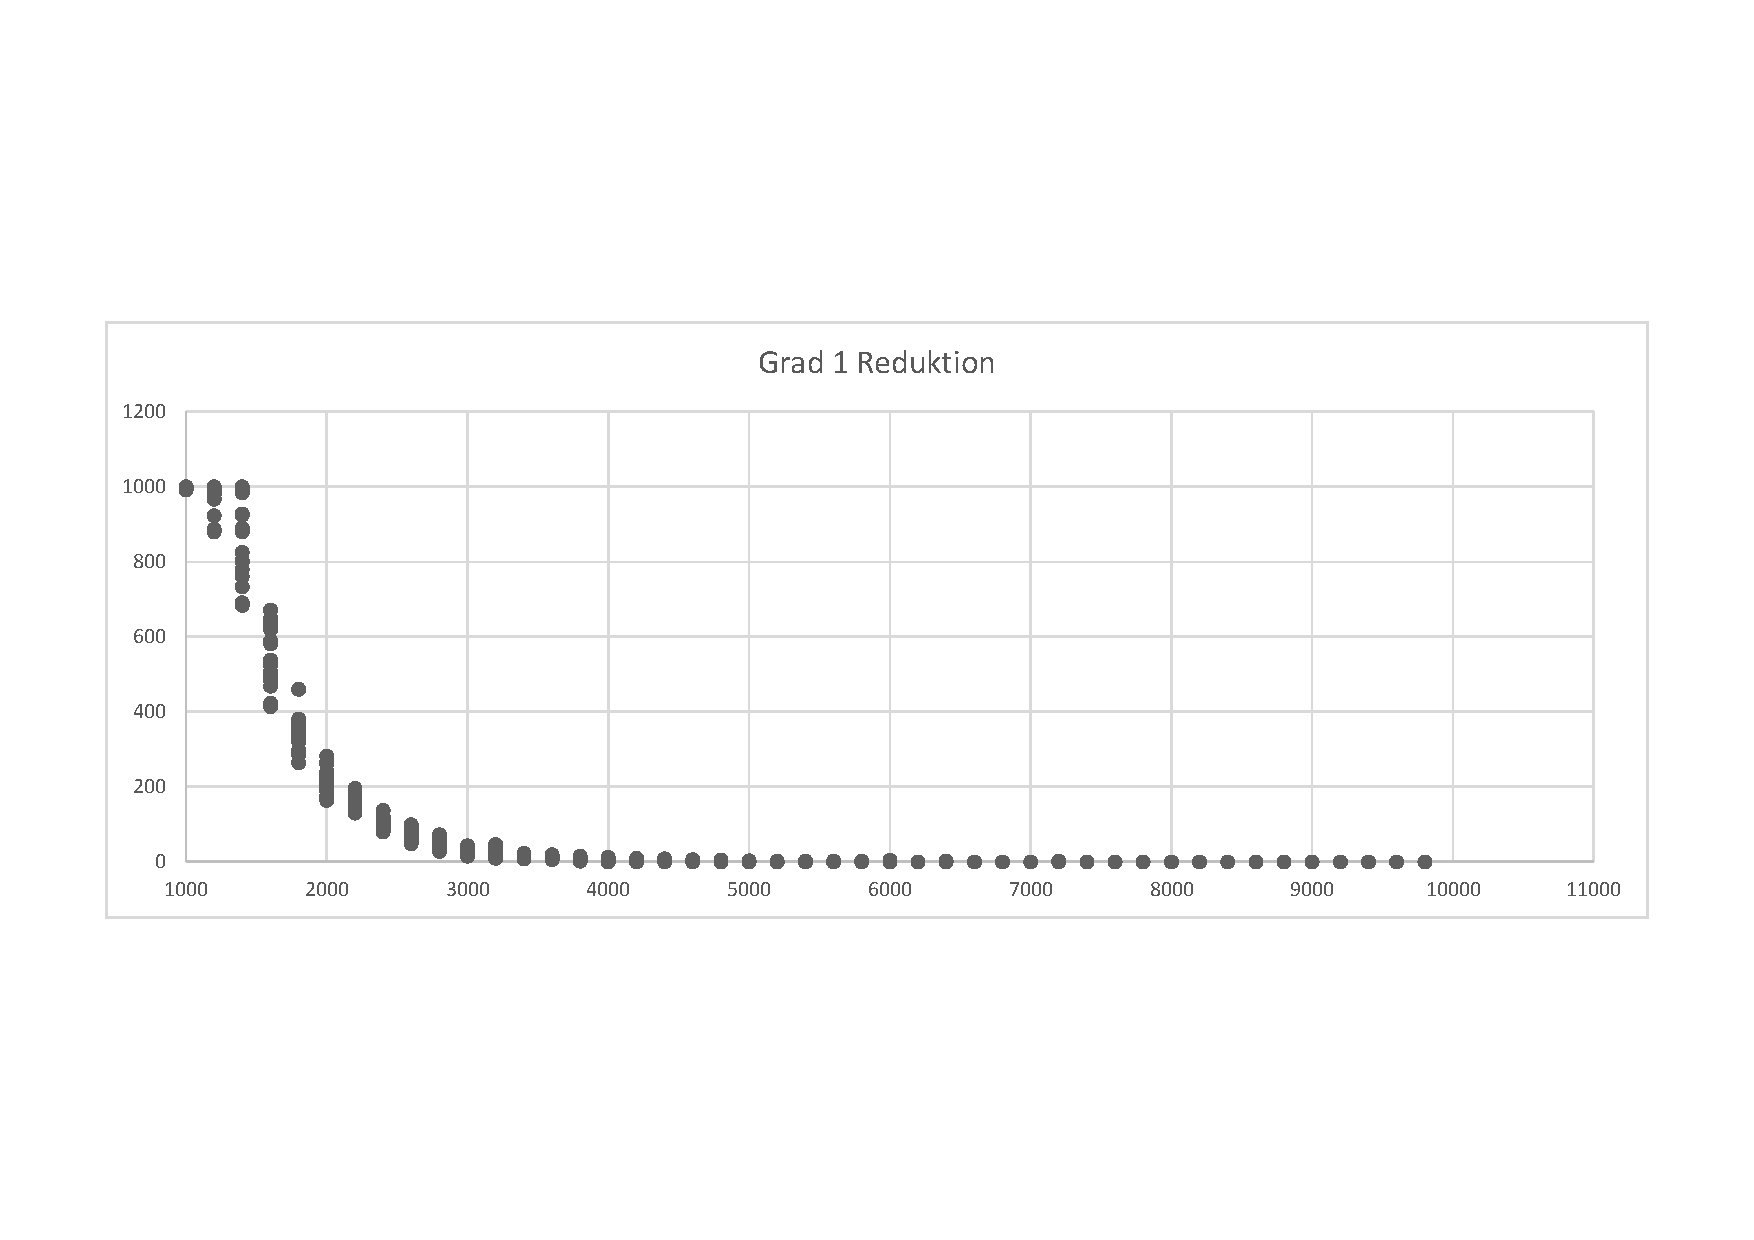
\includegraphics[scale= .4]{analysisOne.pdf} 
\end{frame}

\section{Kronenregel}

\begin{frame}{Kronenregel - Definitionen}
\begin{block}{Krone}\pause
\textit{Für einen Graphen} $G=(V,E)$ \textit{besteht eine Krone aus} $H \subseteq V\ und\ I \subseteq V\ mit\ H \cap I = \emptyset,\ sodass$ \pause
\begin{enumerate}
\item $H = N(I),$ \pause
\item $\forall v, w \in I\ gilt\ (vw) \notin E\ und$\pause
\item \textit{die Kanten zwischen H und I enthalten ein Matching indem alle Knoten aus H enthalten sind.}
\end{enumerate}
\end{block}
\end{frame}

\begin{frame}[fragile]
\frametitle{Kronenregel - Algorithmus}
\begin{lstlisting}[mathescape=true, escapechar = !,basicstyle=\ttfamily\scriptsize]
$G = (V, E), n:= |V|, m:=|E|, d:= maximaler\ Grad\ eines\ Knoten\ aus\ G$!\pause!
$M_{1}$ := Maximal Matching von $G$!\pause!
  $M_{1} := \emptyset$
  $\forall e \in$ E:	!\pause!
    $M_{1} = M_{1} \cup e$ !\pause!
    Entferne $e$ und $N(e)$ aus der weiteren Betrachtung!\pause!
$O$ := nicht gepaarte Knoten in $M_{1}$!\pause!
$M_{2}$ := Maxmimum Matching von $B = (O, N(O), \{ uv| u \in O \wedge v \in N(O)\}) $!\pause!
$I$  := nicht gepaarte Knoten aus $O$ in $M_{2}$!\pause!
$I'  := \emptyset$!\pause!
while $I' \neq I$!\pause!
  $I' := I$!\pause!
  $H:= N(I)$!\pause!
  $I := I \cup \{\forall u \in O|\exists v\in H\ (uv \in M_{2})\}$!\pause!
Entferne $N(I)$ aus $G$!\pause!
\end{lstlisting}
\end{frame}

\begin{frame}[fragile]
\frametitle{Kronenregel - Laufzeit}
\begin{lstlisting}[mathescape=true, escapechar = !,basicstyle=\ttfamily\scriptsize]
$G = (V, E), n:= |V|, m:=|E|, d:= maximaler\ Grad\ eines\ Knoten\ aus\ G$
$M_{1}$ := Maximal Matching von $G$
  $M_{1} := \emptyset$
  $\forall e \in$ E:
    $M_{1} = M_{1} \cup e$
    Entferne $e$ und $N(e)$ aus der weiteren Betrachtung
$O$ := nicht gepaarte Knoten in $M_{1}$
$M_{2}$ := Maxmimum Matching von $B = (O, N(O), \{ uv| u \in O \wedge v \in N(O)\}) $
$I$  := nicht gepaarte Knoten aus $O$ in $M_{2}$
$I'  := \emptyset$
while $I' \neq I$
  $I' := I$
  $H:= N(I)$
  $I := I \cup \{\forall u \in O|\exists v\in H\ (uv \in M_{2})\}$
Entferne $N(I)$ aus $G$
\end{lstlisting}
\only<1>{Zeilen 1-5: $m \cdot d$}
\only<2>{Zeile 6: $n$}
\only<3>{Zeile 7 (1): $n d/2$} % $(n-2k) d/2$
\only<4>{Zeile 7 (2): $\sqrt{n} \cdot m $ (LEDA:mcb\_matching, Hopcroft und Karp) } %$\sqrt{n-2k} \cdot m $
\only<5>{Zeile 8: $n$ } %$n-2k$
\only<6>{Zeilen 10-13: $n \cdot d$}%Nachgucken welche Knoten aus O noch in M2   $(n-2k) \cdot d$
\end{frame}
\begin{frame}{Kronenregel - Laufzeit}
\begin{align*}
&\ m \cdot d + n + n d/2 + \sqrt{n} \cdot m + n  + n \cdot d \\ \pause
=&\ d (m+n) +2 n + nd/2 + \sqrt{n} \cdot m \\ \pause
\Rightarrow &\ O(\sqrt{n} \cdot m)
\end{align*}
\end{frame}

\begin{frame}{Kronenregel - Besonderheiten}
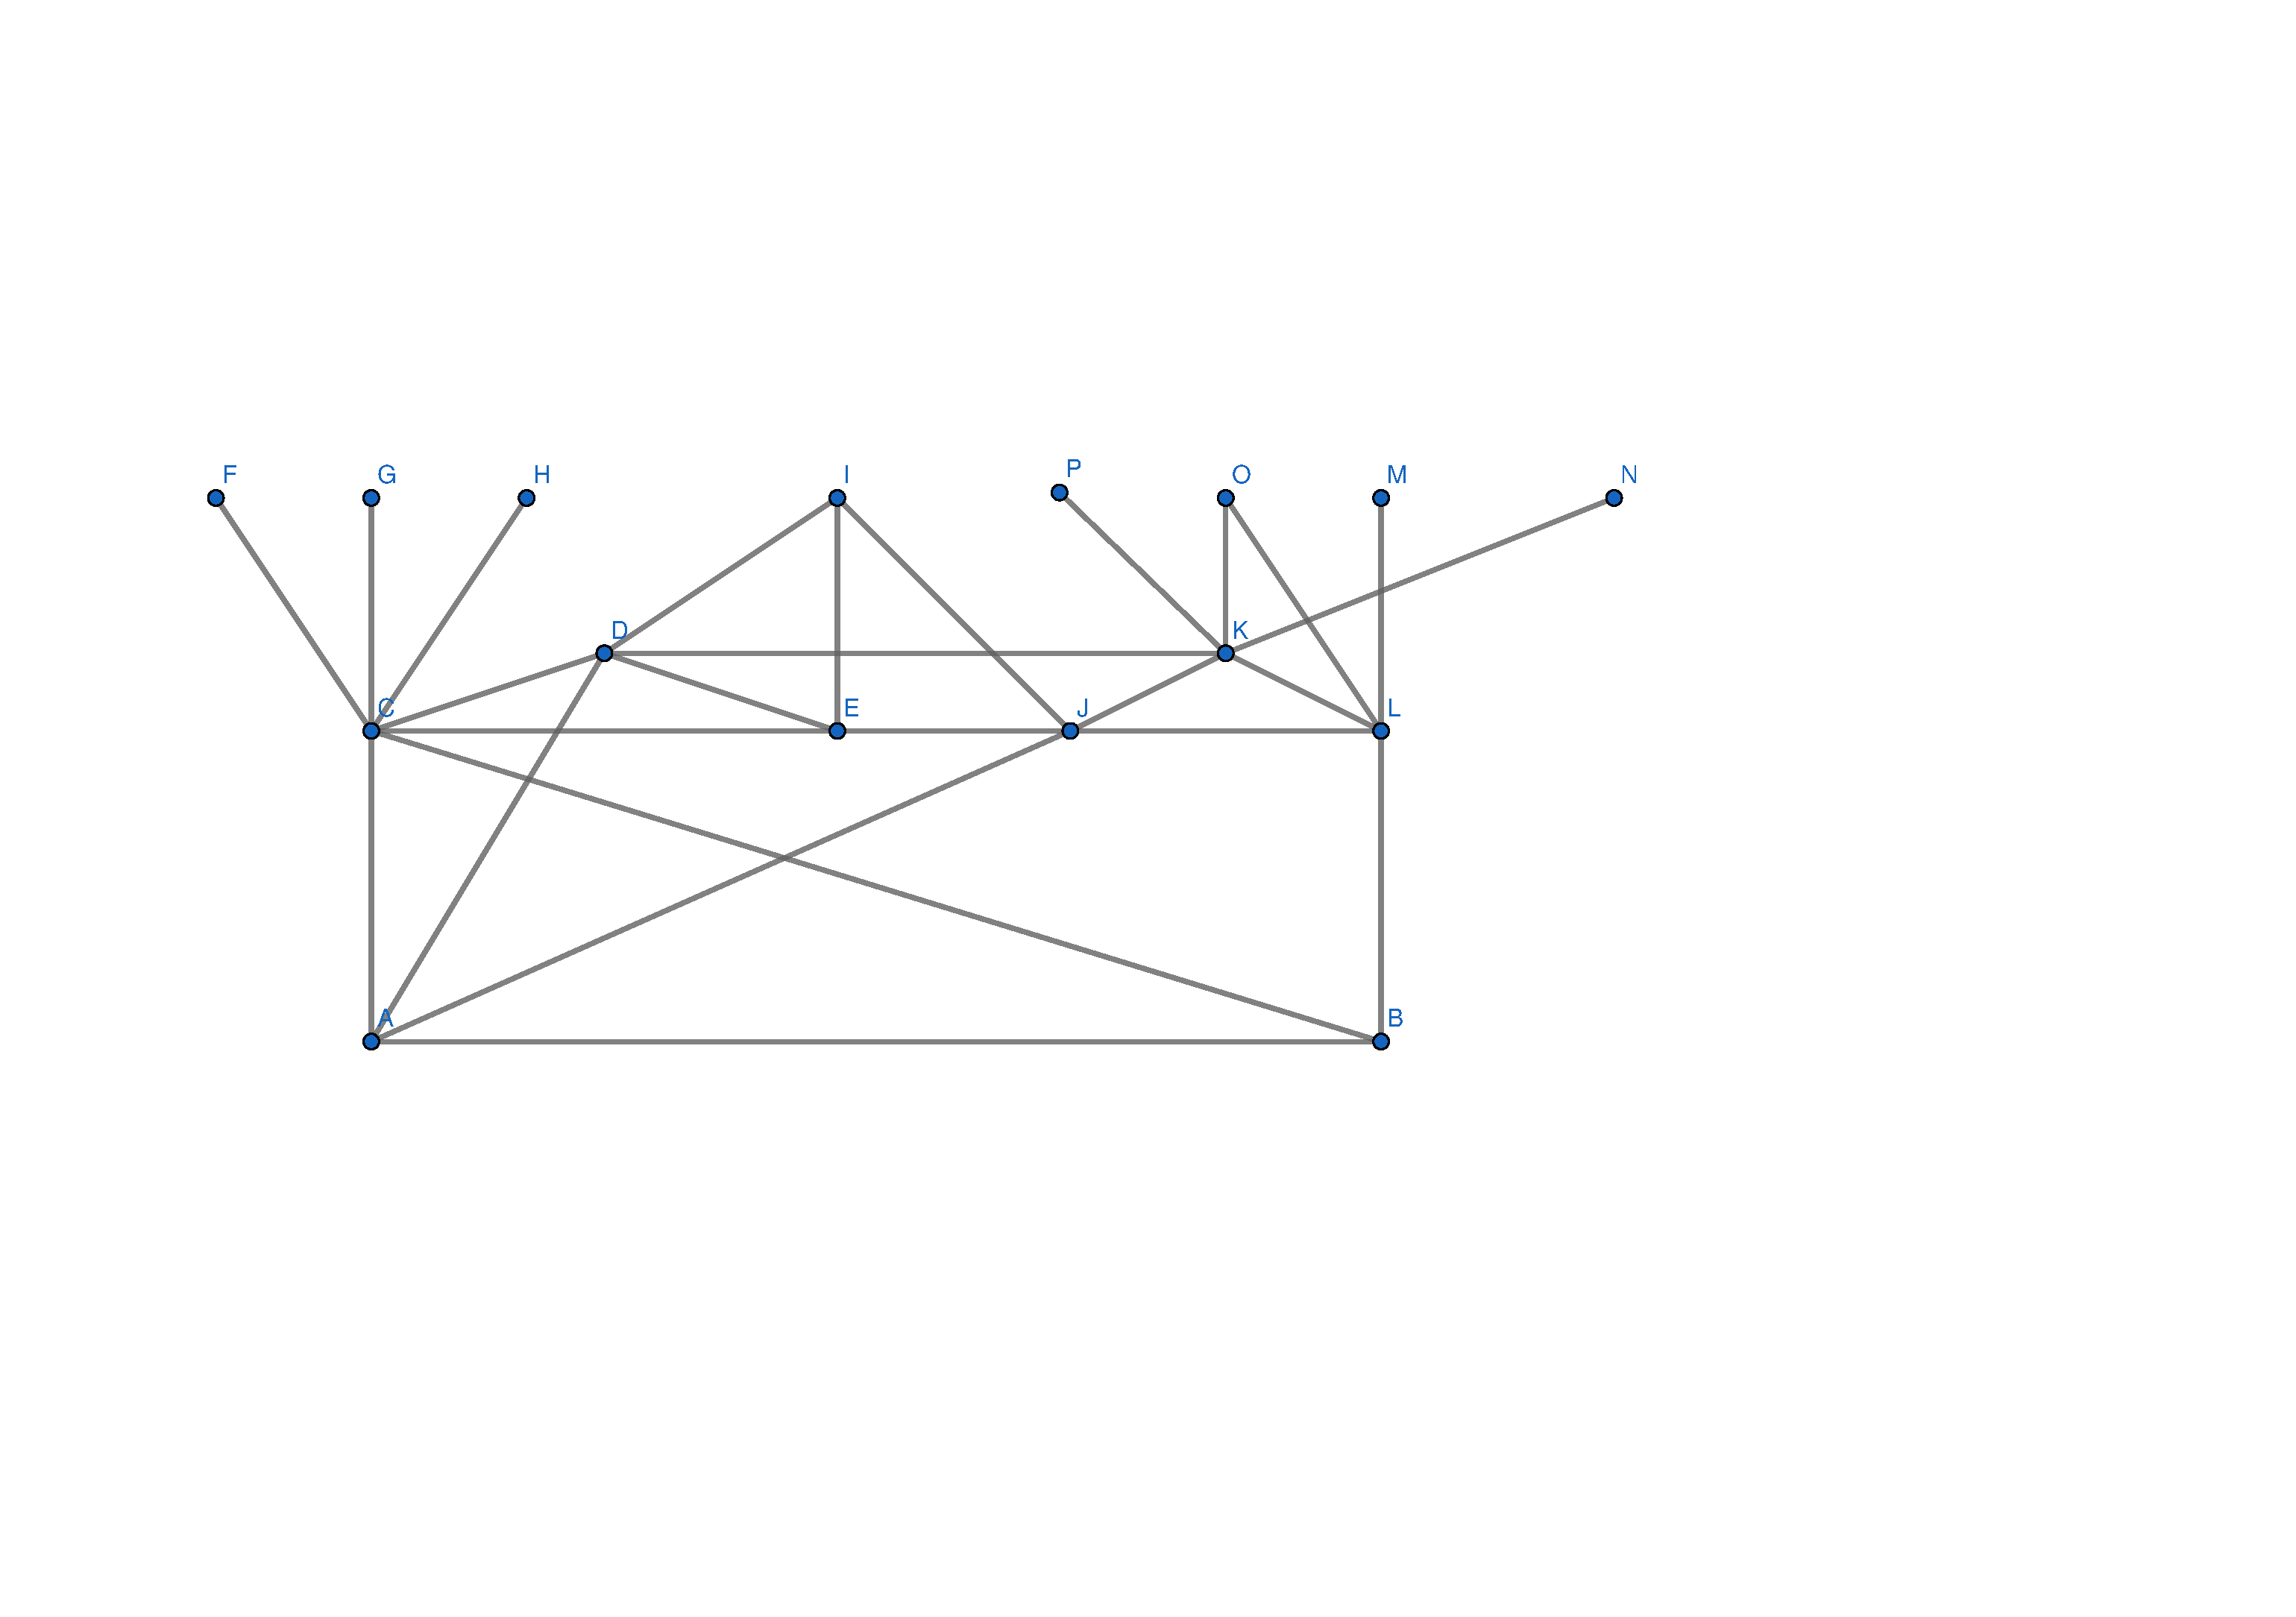
\includegraphics[scale=.3]{Crown1.pdf} 
\end{frame}
\begin{frame}{Kronenregel - Besonderheiten}
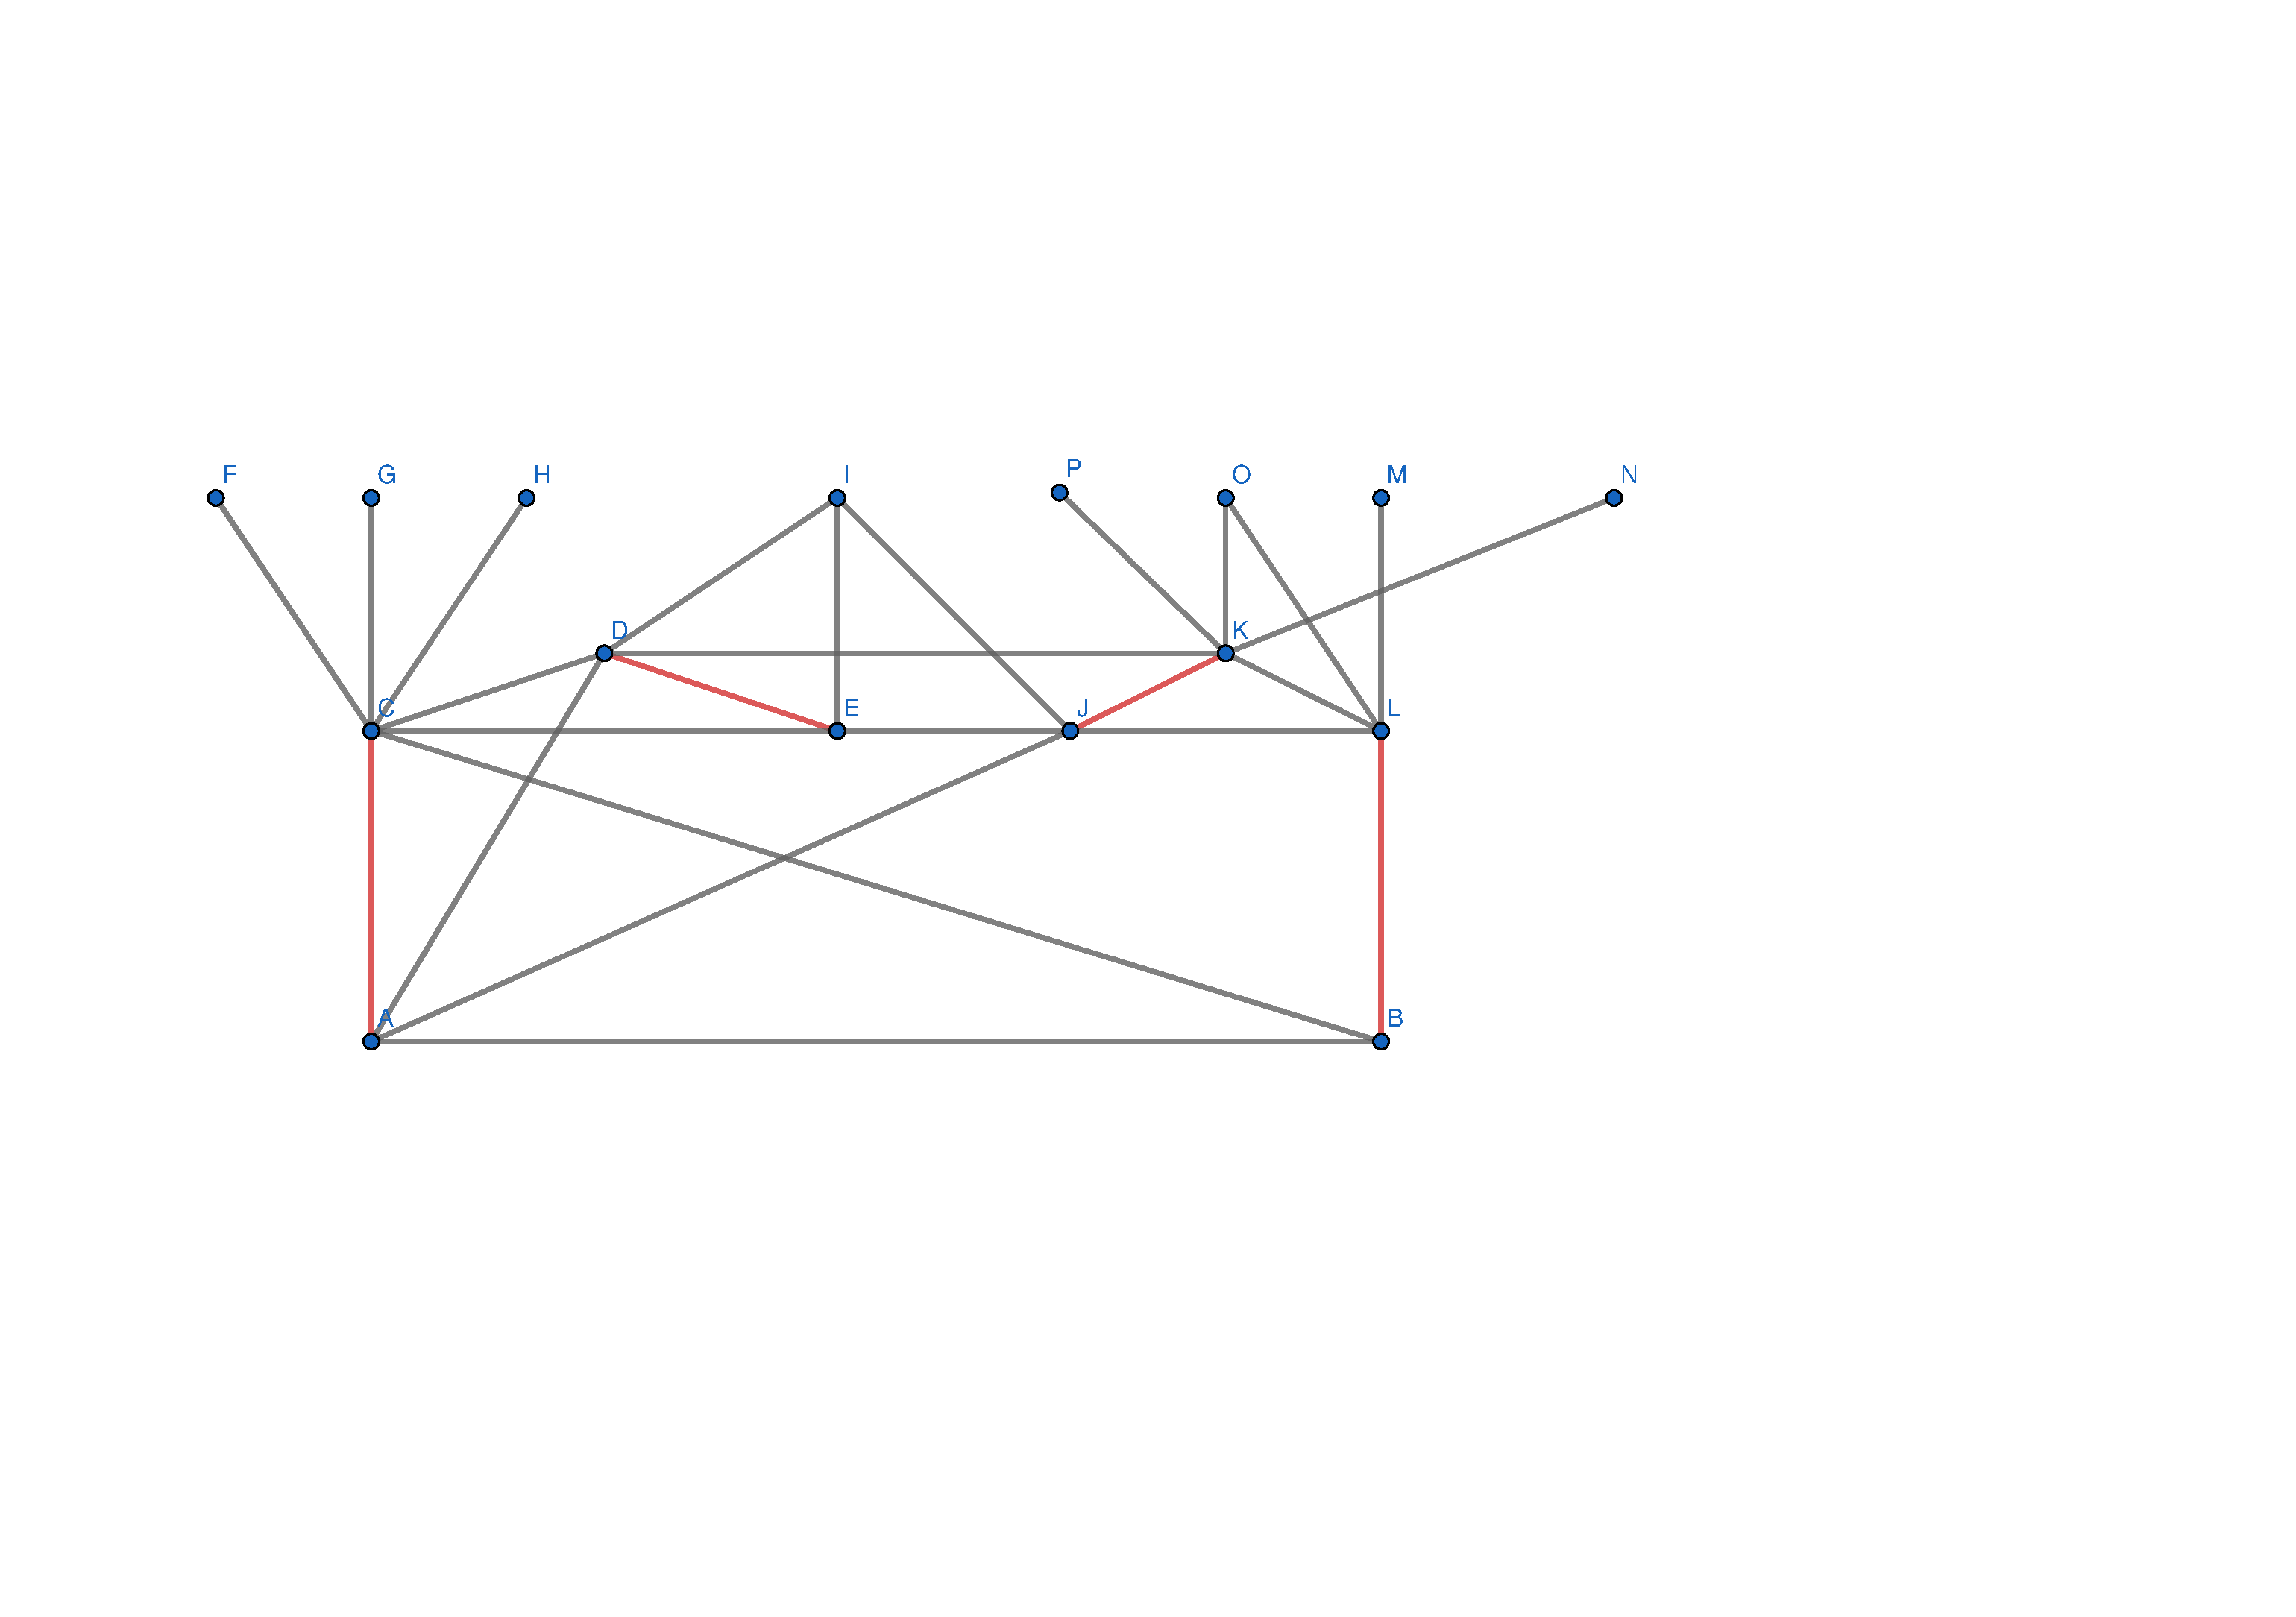
\includegraphics[scale=.3]{Crown2.pdf} 
\end{frame}
\begin{frame}{Kronenregel - Besonderheiten}

\begin{table}[htb]
\caption{Mindestens ein Knoten mit Einschränkung\label{tab:degreeOR}}
\vspace*{1em}
\centering

\bgroup
\def\arraystretch{1.3}%  1 is the default, change whatever you need


\begin{tabular}[c]{l|l|l}
	
	\multicolumn{1}{c|}{\textbf{Grad der Knoten}} & 
	\multicolumn{1}{c|}{\textbf{Anwendungen}} & 
	\multicolumn{1}{c}{\textbf{Reduktion}} \\ 
	
	\hline

	keine Einschränkung&0.29&13.04\\
	$>$1&0.29 &13.04 \\
	$>$2&0.29 &13.22 \\
	$>$3& 0.27& 12.92 \\
	$>$4& 0.3& 13.71 \\
	$>$5& 0.31&13.38 \\ \pause
	Größte Anzahl& 0.32&13.44 \\
	Durchschnittliche Anzahl& 0.29&12.98 \\
	
\end{tabular}


\egroup

\end{table}

\end{frame}



\begin{frame}{Kronenregel - Besonderheiten}
\begin{table}[htb]
\caption{Beide Knoten mit Einschränkung\label{tab:degreeAND}}
\vspace*{1em}
\centering

\bgroup
\def\arraystretch{1.3}%  1 is the default, change whatever you need

\begin{tabular}[c]{l|l|l}
	
	\multicolumn{1}{c|}{\textbf{Grad der Knoten}} & 
	\multicolumn{1}{c|}{\textbf{Anwendungen}} & 
	\multicolumn{1}{c}{\textbf{Reduktion}} \\ 
	
	\hline

	keine Einschränkung&0.29&13.04\\
	$>$1&0.36 &15.34 \\
	$>$2&0.41 &16.96 \\
	$>$3& 0.39& 16.52 \\
	$>$4& 0.4 &15.78 \\
	$>$5& 0.4 & 15.72\\ \pause
	Größte Anzahl& 0.29 &13.06 \\
	Durchschnittliche Anzahl& 0.46&19.77 \\
	
\end{tabular}
\egroup

\end{table}
\end{frame}

\begin{frame}{Kronenegel - Laufzeit}
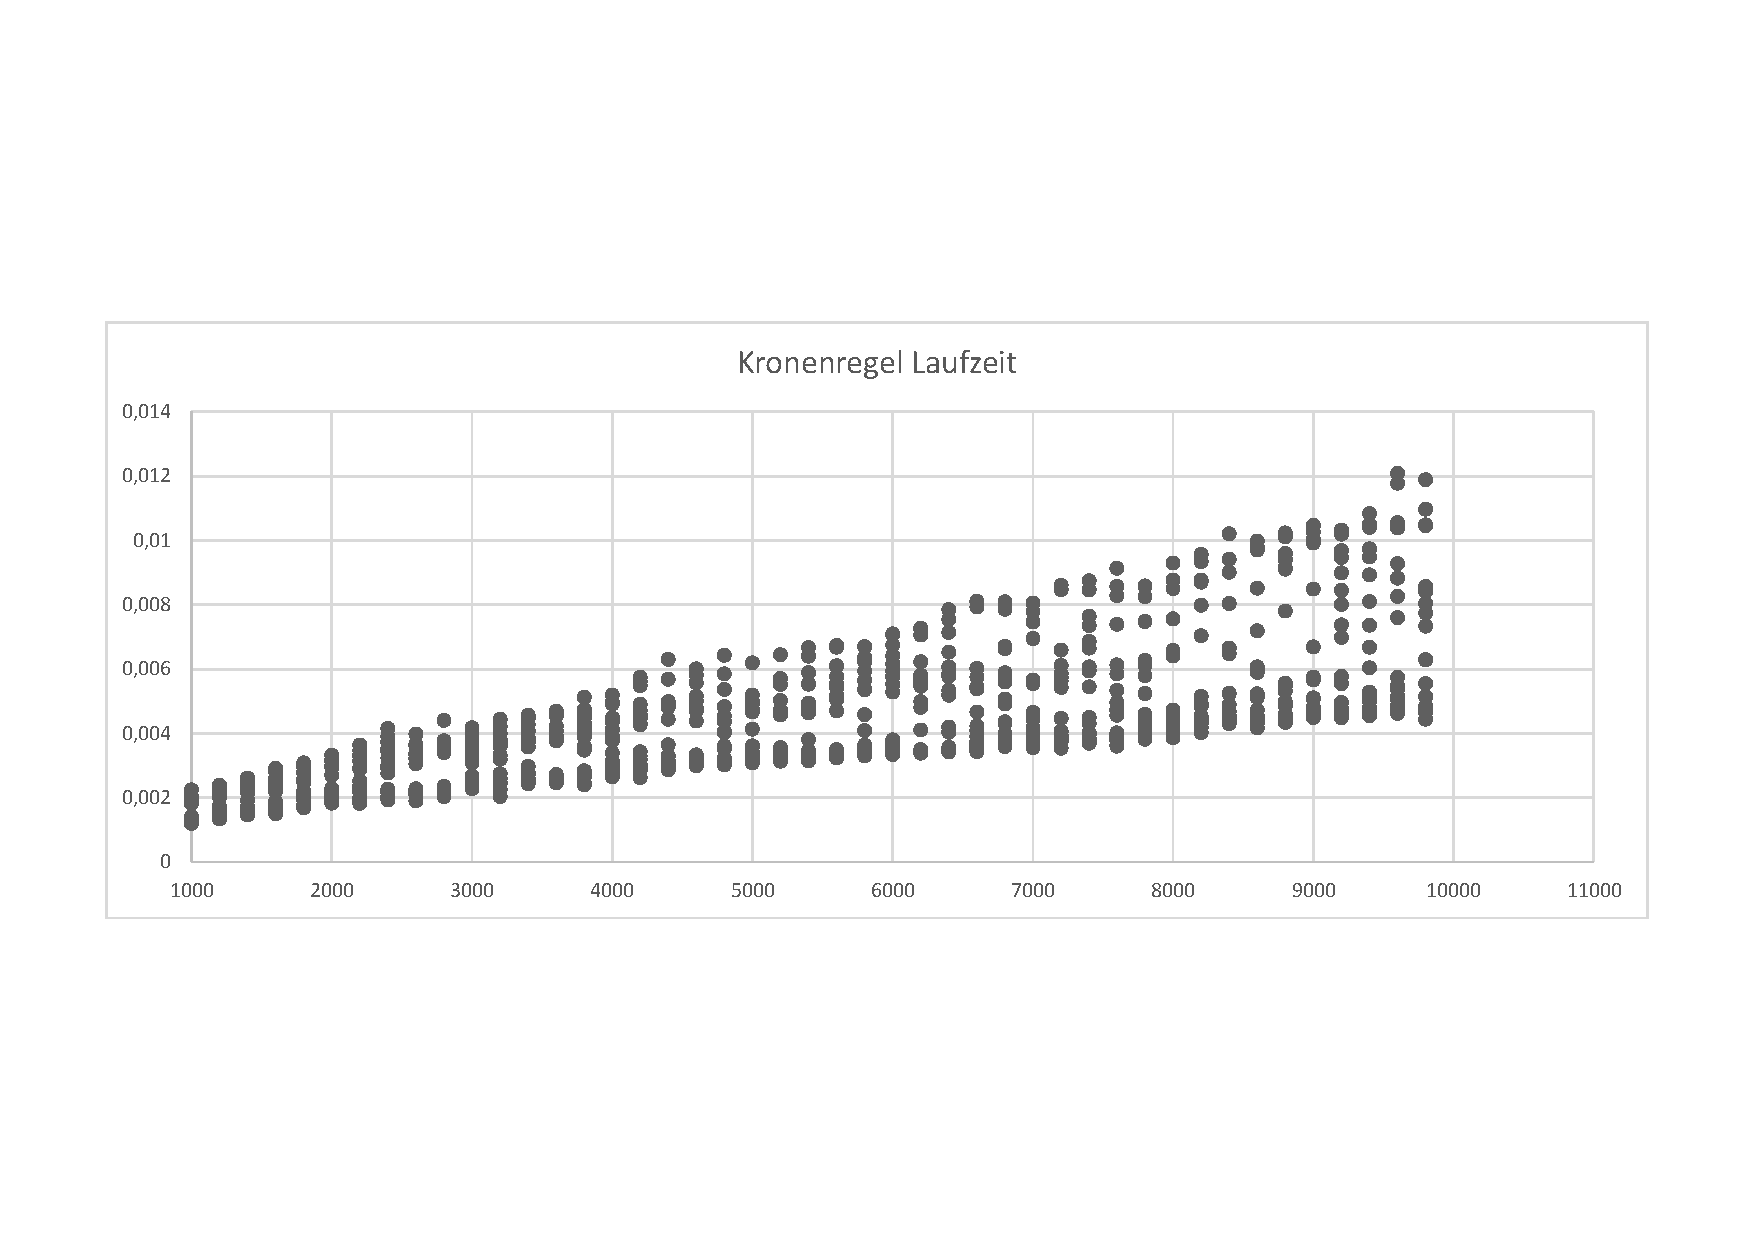
\includegraphics[scale= .4]{analysis1000_CrownNormal_runtime.pdf} 
\end{frame}

\begin{frame}{Kronenregel - Ergebnisse}
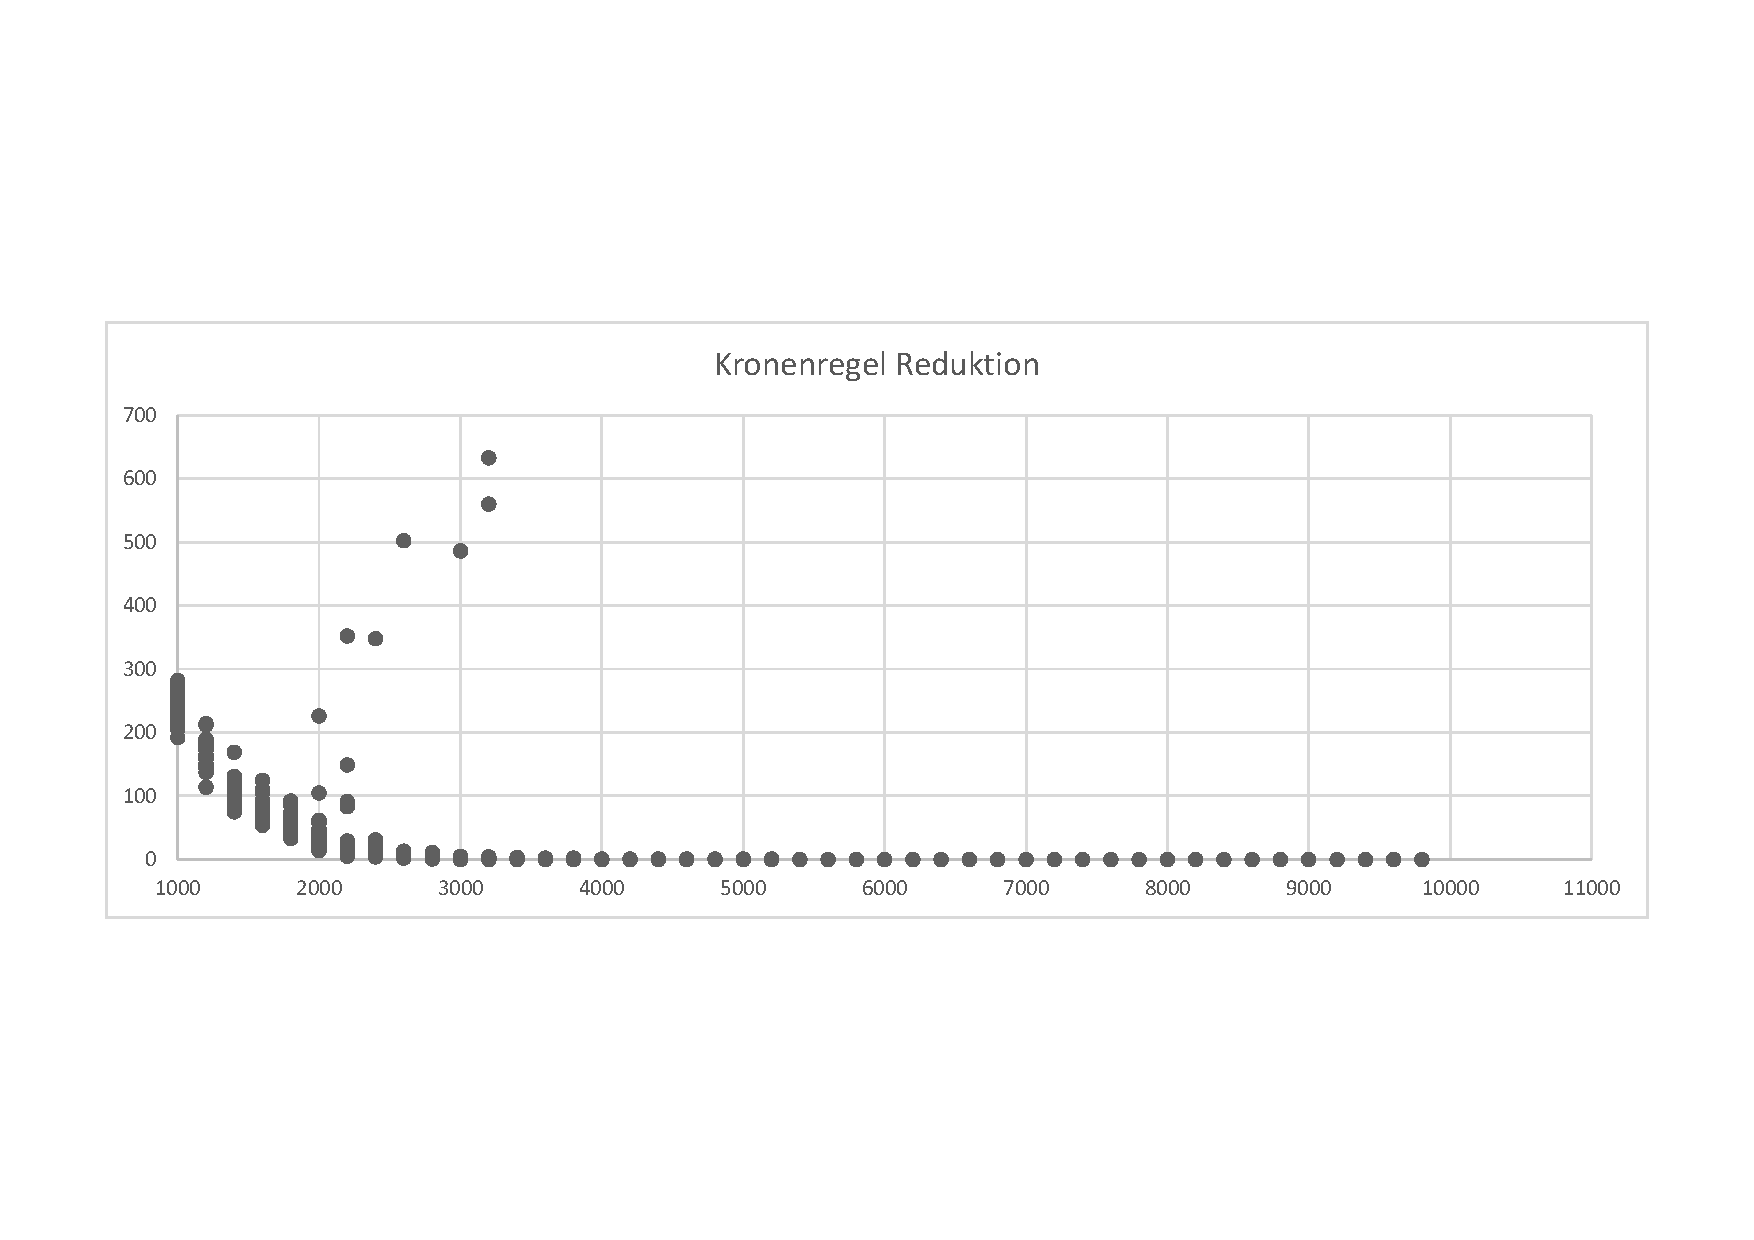
\includegraphics[scale= .4]{analysisCrown.pdf} 
\end{frame}

\section{Nemhauser-Trotter-Regel}
	
\begin{frame}{Nemhauser-Trotter-Regel}
\begin{block}{Nemhauser-Trotter-Theorem}
$\textit{Für einen Graphen}\ G=(V,E)\textit{ können zwei disjunkte Mengen}$\\ $\ C_{0}\ und\ V_{0} \textit{ gefunden werden, sodass}$\pause
\begin{enumerate}
\item $C_{0}$ \textit{ in einer minimalen Knotenüberdeckung} \\
\textit{von G enthalten ist,}\pause
\item \textit{der Teilgraph }$G[V_{0}]$ \textit{eine Knotenüberdeckung}\\
\textit{der Größe} $\leq |V_{0}| / 2$ \textit{ hat,}\pause
\item \textit{und} $VC(G) = VC(G[V_{0}])\cup C_{0}$ \textit{ gilt.}
\end{enumerate}

\end{block}
\end{frame}
	
\begin{frame}[fragile]
\frametitle{NT-Regel - Algorithmus}
\begin{lstlisting}[mathescape = true, basicstyle=\ttfamily, escapechar = !]
$G = (V, E), n:= |V|, m:=|E|, d:= maximaler\ Grad\ eines\ Knoten\ aus\ G$!\pause!
Bipartiden Graphen erstellen $B = (V, V', E')$
  mit $E':= \{\{x,y'\}, \{x', y\} | \{x,y\} \in E\}$!\pause!
Maximum Matching $M$ von $B$ bestimmen!\pause!
$C_{B}:= VC(B)$!\pause!
$C_{0}:= \{x \in V\ |\ x \in C_{B}\ und\ x' \in C_{B} \}$!\pause!
$V_{0}:= \{x \in V\ |\ entweder\ x \in C_{B}\ oder\ x' \in C_{B} \}$
\end{lstlisting}

\end{frame}

\begin{frame}[fragile]
\frametitle{NT-Regel - Laufzeit}
\begin{lstlisting}[mathescape = true, basicstyle=\ttfamily]
$G = (V, E), n:= |V|, m:=|E|, d:= maximaler\ Grad\ eines\ Knoten\ aus\ G$
Bipartiden Graphen erstellen $B = (V, V', E')$ 
  mit $E':= \{\{x,y'\}, \{x', y\} | \{x,y\} \in E\}$ 
Maximum Matching $M$ von $B$ bestimmen 
$C_{B}:= VC(B)$ 
$C_{0}:= \{x \in V\ |\ x \in C_{B}\ und\ x' \in C_{B} \}$ 
$V_{0}:= \{x \in V\ |\ entweder\ x \in C_{B}\ oder\ x' \in C_{B} \}$ 
\end{lstlisting}
\only<1>{Zeilen 1-2: $n \cdot 2d$}
\only<2>{Zeilen 3-4: $\sqrt{n} \cdot m$ (LEDA:mcb\_matching, Hopcroft und Karp)}
\only<3>{Zeilen 5-6: $2n + k \cdot d$}
\end{frame}
\begin{frame}{NT-Regel - Laufzeit}
\begin{align*}
&\ n \cdot 2d + \sqrt{n} \cdot m + 2n + k \cdot d\\ \pause
\Rightarrow &\ O(n + \sqrt{n} \cdot m)
\end{align*}
\end{frame}


\begin{frame}{NT-Regel - Laufzeit}
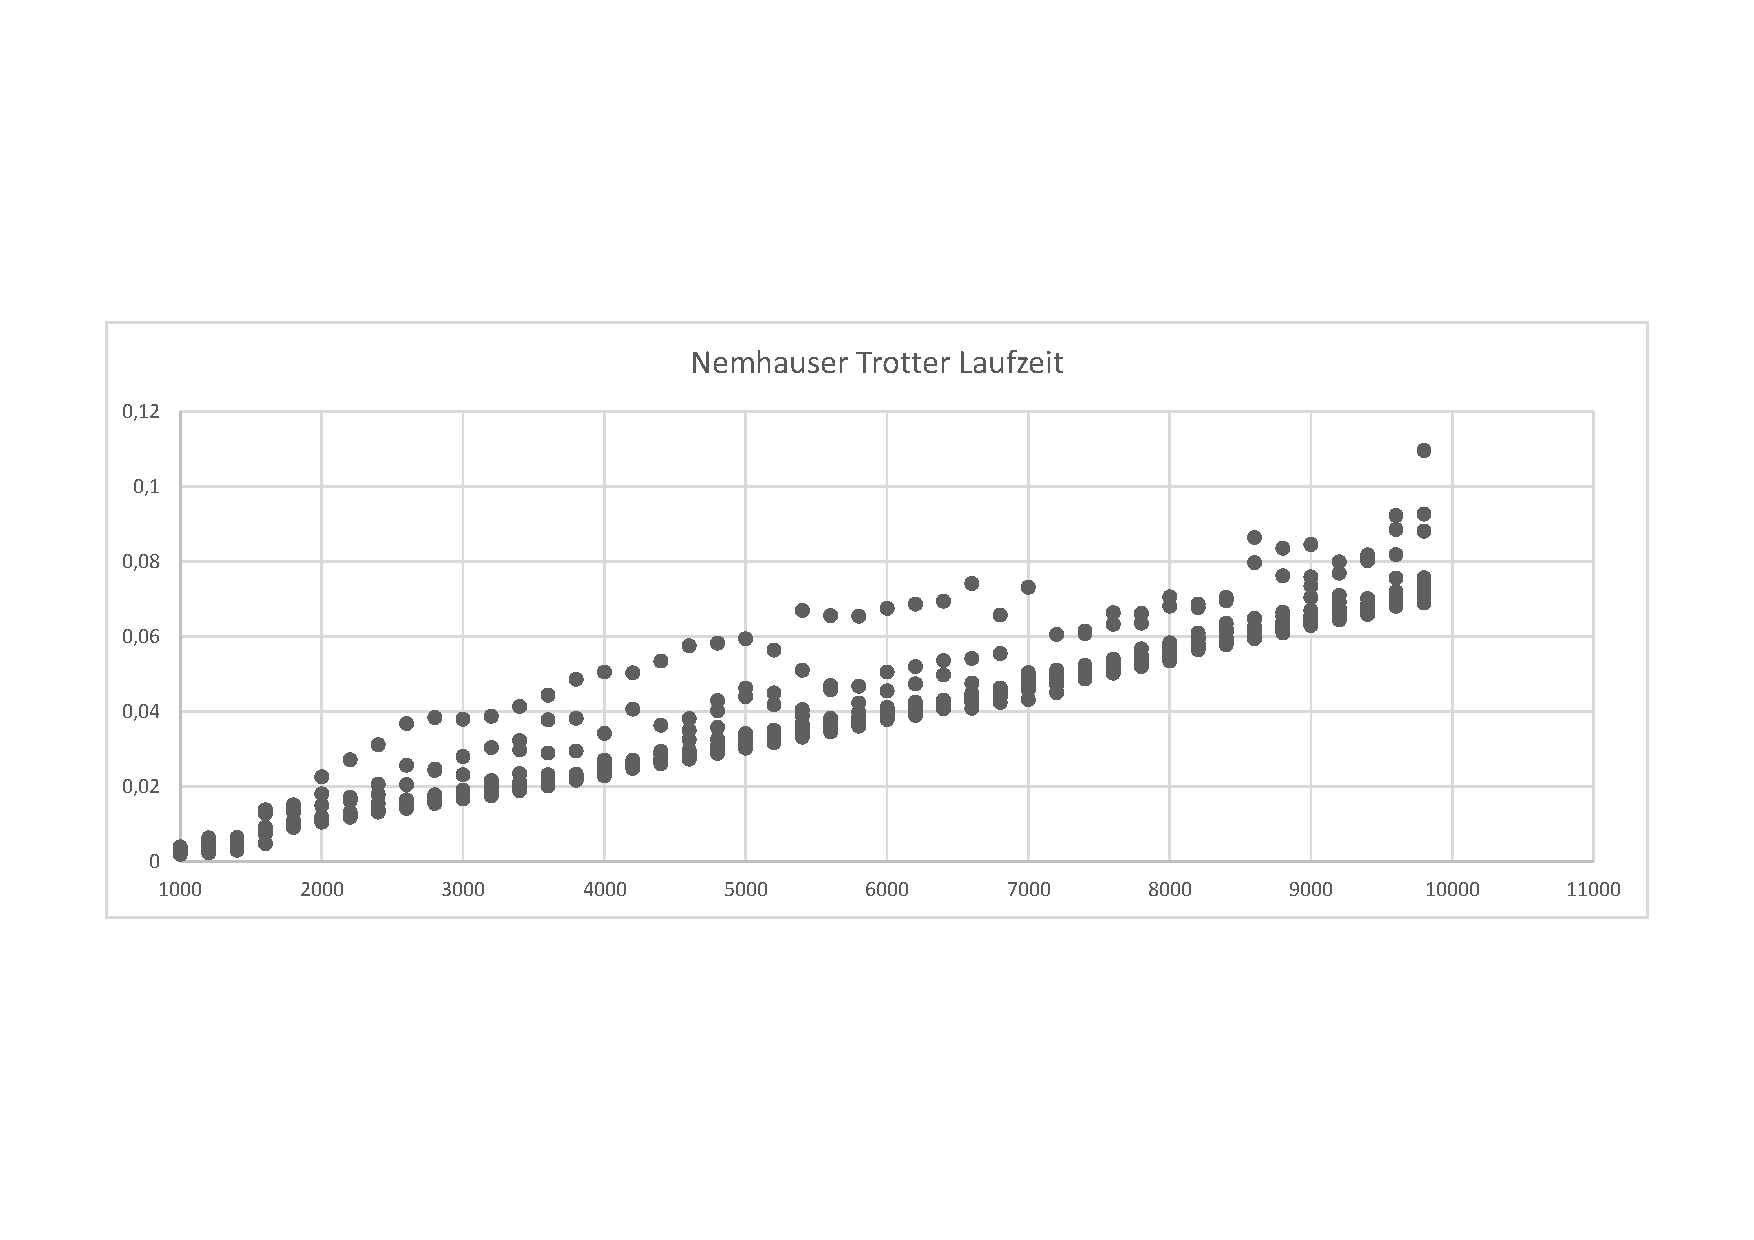
\includegraphics[scale= .4]{analysis1000_TrottNormal_runtime.pdf} 
\end{frame}
\begin{frame}{NT-Regel - Ergebnisse}
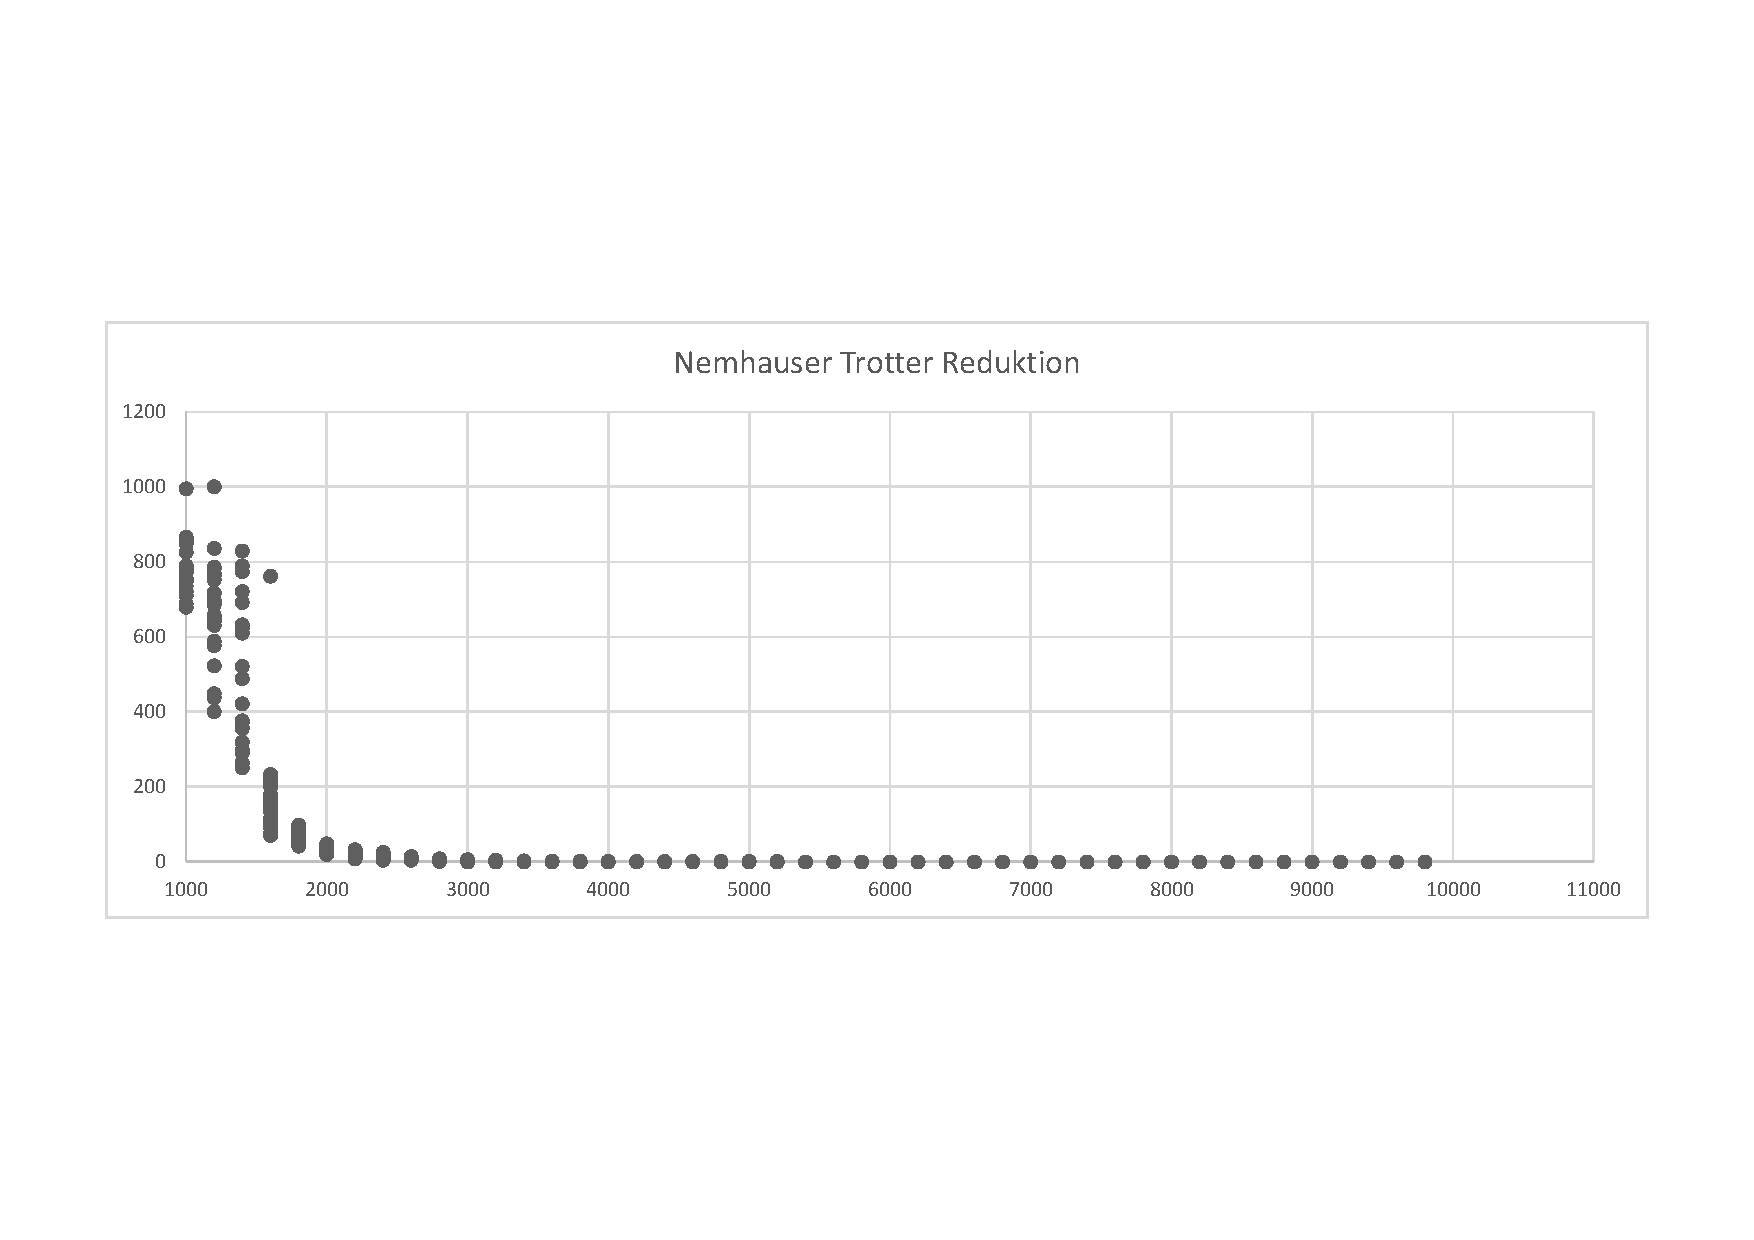
\includegraphics[scale= .4]{analysisTrott.pdf} 
\end{frame}

\section{Vergleich}
\begin{frame}{Vergleich der Ergebnisse}
\begin{table}[htb]
\caption{Anwendung einzelner Reduktionsregeln\label{tab:anwendung}}
\vspace*{1em}
\centering

\bgroup
\def\arraystretch{1.3}%  1 is the default, change whatever you need

\begin{tabular}[c]{llll}
	
	\hline
	\multicolumn{1}{c}{\textbf{Reduktionsregel}} & 
	\multicolumn{1}{c}{\textbf{Anwendungen}} & 
	\multicolumn{1}{c}{\textbf{Reduktion}} & 
	\multicolumn{1}{c}{\textbf{CPU-Zeit }} \\ 
	
	\hline

	Nemhauser-Trotter& 0.27 &  50.3 & 0.041s\\
	Kronenregel& 0.46 & 19.77 & 0.004s\\
	Grad 1&1.32 & 99.06 & 0.0006s\\
	\hline
\end{tabular}
\egroup

\end{table}
\end{frame}

\section{Anwendung}
\begin{frame}{Kombination}
\begin{table}[htbp]
\caption{Anwendung kombinierter Reduktionsregeln\label{tab:kombination}}
\vspace*{1em}
\centering

\bgroup
\def\arraystretch{1.3}%  1 is the default, change whatever you need
\resizebox{\linewidth}{!}{
\begin{tabular}[c]{lllll}

	\hline
	\multicolumn{1}{c}{\textbf{Kombination}} &
	\multicolumn{1}{c}{\textbf{Anwendungen$_{1}$}} &
	\multicolumn{1}{c}{\textbf{Anwendungen$_{2}$}} &
	\multicolumn{1}{c}{\textbf{Anwendungen$_{3}$}} & 
	\multicolumn{1}{c}{\textbf{Reduktion}} \\
	\hline

	K - G$_{1}$ & 3.63 & 4.3 & - &331.8\\
	G$_{1}$ - K & 4.37 & 3.22 & - &331.17\\
	K - NT & 0.8 & 0.38 & - & 68.28 \\
	NT - K & 0.45 & 0.56 & - & 68.6\\
	G$_{1}$ - NT & 1.33 & 0.017 & - & 99.87\\
	NT - G$_{1}$ & 0.28 & 1.13 & - & 99.87\\
	\hline
\end{tabular}
}
\egroup

\end{table}
\end{frame}
	\begin{frame}{Kombination}
\begin{table}[htbp]
\caption{Anwendung kombinierter Reduktionsregeln\label{tab:kombination}}
\vspace*{1em}
\centering

\bgroup
\def\arraystretch{1.3}%  1 is the default, change whatever you need
\resizebox{\linewidth}{!}{
\begin{tabular}[c]{lllll}

	\hline
	\multicolumn{1}{c}{\textbf{Kombination}} &
	\multicolumn{1}{c}{\textbf{Anwendungen$_{1}$}} &
	\multicolumn{1}{c}{\textbf{Anwendungen$_{2}$}} &
	\multicolumn{1}{c}{\textbf{Anwendungen$_{3}$}} & 
	\multicolumn{1}{c}{\textbf{Reduktion}} \\
	\hline
	
	K  - G$_{1}$ - NT & 3.61 & 4.29 & 0.11 & 334.67 \\
	K - NT - G$_{1}$ & 3.6 & 0.87 & 3.39 & 334.83 \\
	G$_{1}$ - NT - K & 4.36 & 0.12 & 3.2 & 334.17 \\
	G$_{1}$ - K - NT & 3.61 & 3.2 & 0.65 & 334.16 \\
	NT - K - G$_{1}$ & 0.39 & 3.44 & 4.03 & 335.2 \\
	NT - G$_{1}$ - K & 0.91 & 3.42 & 3.2 & 334.16 \\
	\hline
	
\end{tabular}
}
\egroup
\end{table}
\end{frame}

\begin{frame}{Kombination}
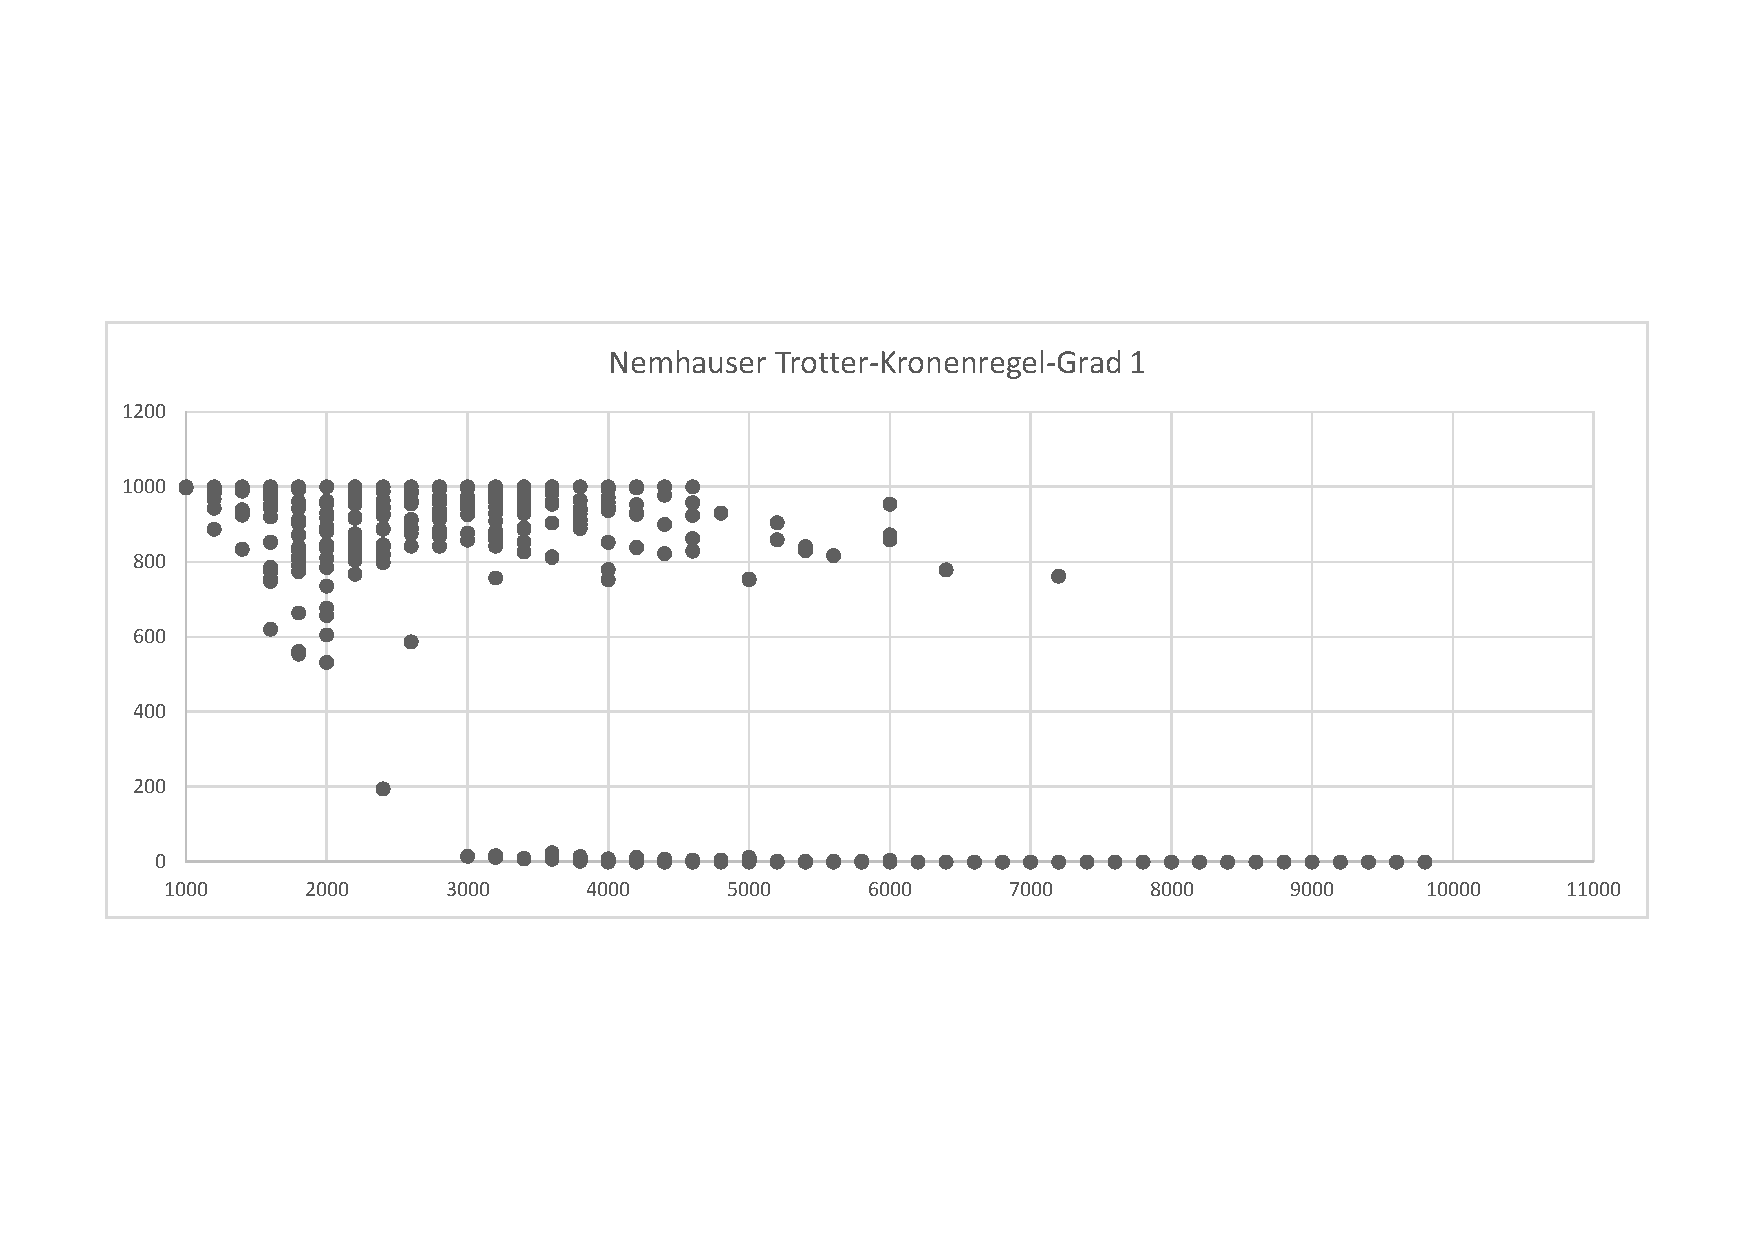
\includegraphics[scale=.4]{analysisTrott_Crown_One.pdf} 
\end{frame}

\begin{frame}{Kombination}
\begin{table}[htb]
\caption{Besondere Graphen für die Dreierkombinationen von Regeln\label{tab:trottCrownOneSpecial}}
\vspace*{1em}
\centering

\bgroup
\def\arraystretch{1.3}%  1 is the default, change whatever you need
\resizebox{\linewidth}{!}{
\begin{tabular}[c]{llllll}
	\hline
	\multicolumn{1}{c}{\textbf{Graph}} & 
	\multicolumn{1}{c}{\textbf{Reduktionsregeln}} & 
	\multicolumn{1}{c}{\textbf{Anwend.$_{1}$}} &
	\multicolumn{1}{c}{\textbf{Anwend.$_{2}$}} &
	\multicolumn{1}{c}{\textbf{Anwend.$_{3}$}} &
	\multicolumn{1}{c}{\textbf{Reduktion}} \\ 
	
	\hline
		
	Graph$_{1}$ & NT - K - G$_{1}$ & 1 & 5 & 6 & 195 \\
	& G$_{1}$ - NT - K & 6 & 0 & 5 & 195 \\
	& Nemhauser-Trotter & 1 & - & - & 11 \\
	& Kronenregel & 1 & - & - & 11 \\
	& Grad$_{1}$ & 2 & - & - & 91 \\
	& Kronenregel - Grad$_{1}$ & 6 & 5 & - & 195 \\
	
	\hline

	Graph$_{2}$ & NT - K - G$_{1}$ & 1 & 9 & 2 & 762 \\
	& Nemhauser-Trotter & 0 & - & - & 0\\
	& Kronenregel & 0 & - & - & 0\\
	& Grad$_{1}$ & 1 & - & - & 2 \\
	& Kronenregel - Grad$_{1}$ & 9 & 3 & - & 762\\
	\hline
	
\end{tabular}
}
\egroup

\end{table}

\end{frame}


\section{Fazit und Ausblick}
\begin{frame}{Ausblick}
\begin{itemize}
\item Form von randomgraphen untersuchen
	\begin{itemize}
	\item Welche Form hinterlassen die Reduktionsregeln
	\item Welche Form wäre für die Nemhauser Trotter am besten
	\end{itemize}
\item Warum ist die Nemhauser-Trotter-Regel in der Praxis so schlecht?
\item Wie ergibt sich in bei den Reduktionen (Abbildung \ref{fig:trottCrownOne}) der Große Unterschied zwischen den Graphen im Bereich der Kantenmenge zwischen 3000 und 4600?
\item Wieso ist das Matching M1 so wichtig für die Kronenregel?
\end{itemize}
\end{frame}
  \begin{frame}[allowframebreaks]
        \frametitle{Quellen}
         % nur angeben, wenn auch nicht im Text zitierte Quellen 
           % erscheinen sollen
\bibliographystyle{ieeetran}
        \bibliography{thesis.bib}
\end{frame}
\end{document}